% !TEX root = ../../tcc.tex

\chapter{Proposta do Cognita}

% Evita o espaçamento vertical esticado quando tabelas fixas [H] vão para a página seguinte.
\raggedbottom

% Macros locais deste capítulo --------------------------------------------
% Espaço reservado para figuras ainda não produzidas. Para inserir a figura
% final, troque \espacofigura{...} por \includegraphics[width=\textwidth]{figuras/arquivo}.
\newcommand{\espacofigura}[2][6cm]{%
  \fbox{\parbox[c][#1][c]{0.94\textwidth}{\centering\textit{#2}}}}

% Texto ainda a ser escrito (aparece destacado no PDF para não passar despercebido).
\newcommand{\espacotexto}[1]{\par\noindent\textit{#1}\par}
% ---------------------------------------------------------------------------

Este capítulo documenta o planejamento do Cognita, módulo de previsão de
conhecimento a ser incorporado ao Ecossistema CEDIS. A
Seção~\ref{sec:visao-produto} apresenta a visão do produto e os resultados
da \textit{Lean Inception}; a Seção~\ref{sec:requisitos} reúne os requisitos
funcionais e não funcionais, organizados em temas e épicos, e delimita o
escopo do MVP e dos incrementos; a
Seção~\ref{sec:arquitetura} documenta a arquitetura atual do ecossistema e a
arquitetura proposta para o módulo; a Seção~\ref{sec:modelagem-dados}
descreve as entidades e os atributos do ecossistema que alimentarão o
Cognita; a Seção~\ref{sec:prototipacao} apresenta a prototipação das
telas; e a Seção~\ref{sec:cronograma} apresenta o cronograma de
desenvolvimento por ondas.


\section{Visão do Produto}
\label{sec:visao-produto}

Esta seção sintetiza os artefatos da \textit{Lean Inception} que sustentam
o restante do planejamento. Os detalhes dos \textit{workshops} não são
reproduzidos aqui; registram-se apenas os resultados que orientam a
definição dos requisitos.

\subsection{Visão e Escopo}
\label{subsec:visao-escopo}

\espacotexto{Futuramente será apresentada a declaração de visão do produto e o quadro ``É / Não é / Faz / Não faz'' produzidos na \textit{Lean Inception}.}

\subsection{Personas}
\label{subsec:personas}

\espacotexto{Futuramente serão apresentadas as personas definidas na \textit{Lean Inception}, com perfil, necessidades e dores, às quais as histórias de usuário da Seção~\ref{sec:requisitos} farão referência.}

\subsection{MVP Canvas}
\label{subsec:mvp-canvas}

A Figura~\ref{fig:mvp-canvas} consolida o MVP Canvas do Cognita.

\begin{figure}[H]
\caption{MVP Canvas do Cognita}
\label{fig:mvp-canvas}
\centering
\espacofigura[7cm]{Futuramente será inserido o MVP Canvas produzido na \textit{Lean Inception}}
\legend{Fonte: Dos autores.}
\end{figure}


\section{Requisitos}
\label{sec:requisitos}

Os requisitos do Cognita foram fundamentados nas jornadas de usuário,
descritas na Seção~\ref{sec:visao-produto}. A partir delas, foi realizada
uma fase de \textit{brainstorming} de funcionalidades, conduzida de forma a
contemplar todo o fluxo da jornada dos usuários.

Os requisitos resultantes foram, então, validados por meio de
\textit{feedbacks} de Sérgio Freitas, dono do Ecossistema CEDIS e cliente do
projeto, e submetidos à fase de Revisão Técnica, de Negócio e de UX da
\textit{Lean Inception} \cite{caroli_lean_2018}
(Seção~\ref{subsubsec:lean-inception}). Nessa fase, cada requisito foi
avaliado quanto à viabilidade técnica, ao valor agregado e à experiência do
usuário. O resultado é apresentado na
Figura~\ref{fig:requisitos-priorizacao}.

\begin{figure}[H]
\caption{Requisitos do Cognita avaliados na Revisão Técnica, de Negócio e de UX}
\label{fig:requisitos-priorizacao}
\centering
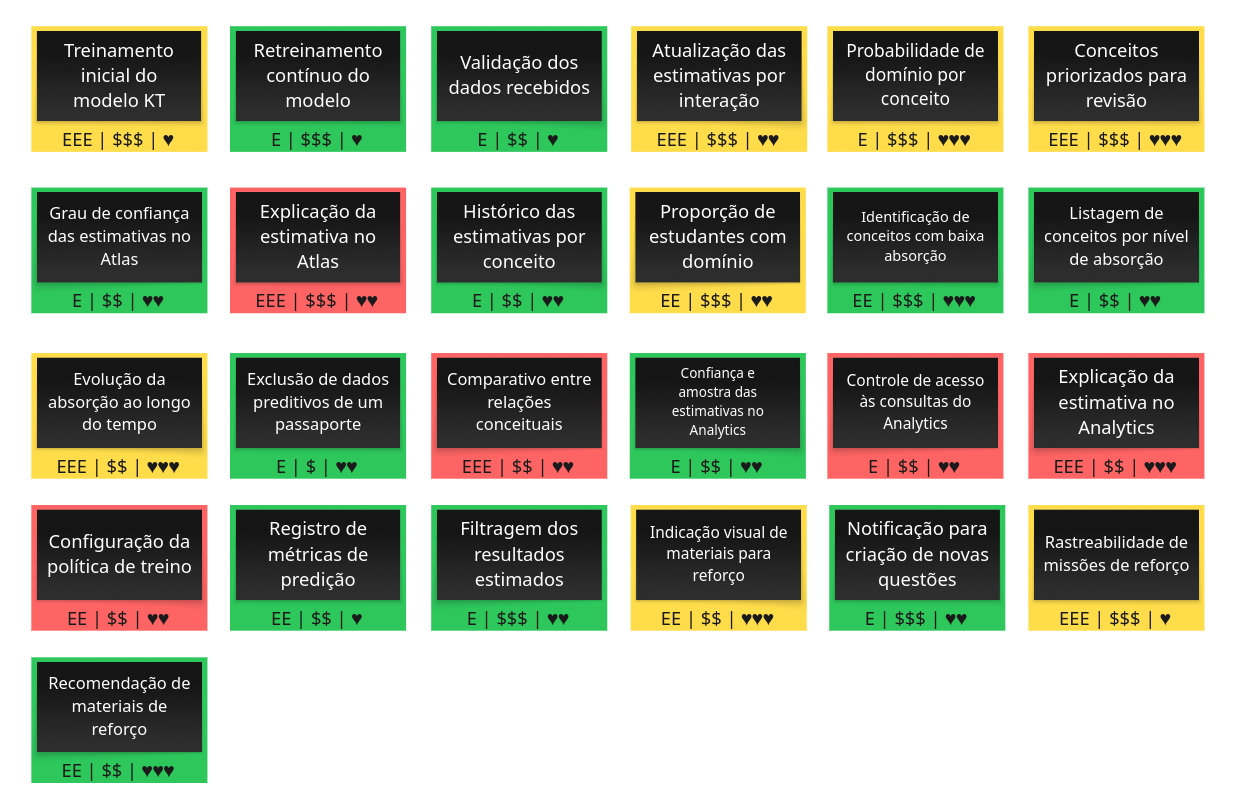
\includegraphics[width=\textwidth]{figuras/requisitos.png}
\legend{Fonte: Dos autores.}
\end{figure}

Cada cartão da figura representa um requisito e é avaliado por quatro
indicadores. A cor indica a aplicabilidade do requisito para os
desenvolvedores: vermelho representa difícil aplicabilidade, amarelo, média
aplicabilidade, e verde, fácil aplicabilidade. Ela foi definida em conjunto
pelos autores, considerando o entendimento do requisito e a facilidade de
implementá-lo. O símbolo \textit{E} indica o nível de esforço necessário
para implementar o requisito, também estimado em conjunto com os
desenvolvedores. Já o símbolo \$ indica o nível de valor agregado ao
produto, e o símbolo $\heartsuit$ indica o nível de contribuição do
requisito para a experiência do usuário (\textit{UX}). Em cada um desses
três indicadores, a quantidade de símbolos varia de um a três, do menor ao
maior nível.

O valor agregado e a experiência do usuário foram definidos por Sérgio
Freitas, por meio de um formulário submetido com todos os requisitos, no
qual os níveis eram escolhidos com base na descrição de cada
requisito.%
\footnote{Formulário disponível em: \textit{[inserir link do formulário]}.}

\subsection{Temas, Épicos e Requisitos Funcionais}
\label{subsec:requisitos-funcionais}

Após a validação na fase de Revisão Técnica, de Negócio e de UX, os
requisitos foram detalhados pelos próprios desenvolvedores, com base no
entendimento do produto construído ao longo de toda a \textit{Lean
Inception}. Esse detalhamento seguiu uma estrutura hierárquica de temas,
épicos e histórias de usuário: os temas agrupam as grandes áreas de valor do
produto, os épicos decompõem cada tema em objetivos funcionais coesos e as
histórias de usuário descrevem cada requisito.

Concluído o detalhamento, Sérgio Freitas validou novamente os requisitos,
avaliando se contemplavam o que era esperado e se não havia ambiguidade em
sua própria interpretação. A versão validada pode ser consultada nas
tabelas de temas (Tabela~\ref{tab:temas}), de épicos
(Tabela~\ref{tab:epicos}) e de requisitos funcionais
(Tabela~\ref{tab:requisitos-funcionais}).

% Futuramente: temas definidos na Lean Inception.
\begin{table}[H]
\caption{Temas do Cognita}
\label{tab:temas}
\centering
\begin{tabularx}{\textwidth}{l>{\raggedright\arraybackslash}p{3.2cm}>{\raggedright\arraybackslash}X}
\hline
\textbf{Código} & \textbf{Título} & \textbf{Descrição} \\
\hline
TM01 & Módulo Cognita & Módulo de previsão de conhecimento incorporado ao Ecossistema CEDIS, que estima o domínio conceitual dos estudantes e entrega diagnósticos acionáveis a eles e aos docentes. \\
\hline
\end{tabularx}
\legend{Fonte: Dos autores.}
\end{table}

% Futuramente: épicos definidos na Lean Inception.
{\small
\begin{longtable}{>{\raggedright\arraybackslash}p{1.4cm}>{\raggedright\arraybackslash}p{2.0cm}>{\raggedright\arraybackslash}p{3.4cm}>{\raggedright\arraybackslash}p{7.0cm}}
\caption{Épicos do Cognita}
\label{tab:epicos} \\
\hline
\textbf{Código} & \textbf{Tema associado} & \textbf{Título} & \textbf{História de usuário} \\
\hline
\endfirsthead
\caption[]{Épicos do Cognita (continuação)} \\
\hline
\textbf{Código} & \textbf{Tema associado} & \textbf{Título} & \textbf{História de usuário} \\
\hline
\endhead
\hline
\multicolumn{4}{r}{\textit{Continua na próxima página}} \\
\endfoot
\hline
\multicolumn{4}{l}{Fonte: Dos autores.} \\
\endlastfoot
EP01 & TM01 & Gestão do modelo preditivo & O sistema deverá treinar, validar, configurar e monitorar o modelo preditivo de forma contínua, para que as estimativas de domínio sejam geradas a partir de dados consistentes e de um modelo confiável. \\
\hline
EP02 & TM01 & Diagnóstico individual de domínio & O estudante deverá acompanhar, no Atlas, o seu domínio de cada conceito, atualizado a cada interação e com a priorização dos conceitos a revisar, para que direcione os seus estudos de forma eficiente. \\
\hline
EP03 & TM01 & Evolução do domínio ao longo do tempo & O professor deverá observar a evolução da absorção dos conceitos de um curso ao longo do tempo, para que avalie o efeito das ações pedagógicas adotadas. \\
\hline
EP04 & TM01 & Diagnóstico de domínio da turma e do curso & O professor deverá analisar, no Analytics, o domínio dos estudantes por conceito de um curso, para que identifique os conceitos críticos e direcione o planejamento das suas ações. \\
\hline
EP05 & TM01 & Transparência das estimativas & O estudante e o professor deverão visualizar o grau de confiança e os motivos das estimativas de domínio, para que compreendam o diagnóstico e confiem nele ao tomar decisões. \\
\hline
EP06 & TM01 & Reforço da aprendizagem & O estudante e o professor deverão contar com ações de reforço voltadas aos conceitos mal absorvidos, para que as dificuldades de aprendizado sejam superadas. \\
\hline
EP07 & TM01 & Privacidade e controle de acesso & O usuário deverá ter os seus dados preditivos protegidos por regras de acesso e pela possibilidade de exclusão, para que a sua privacidade seja preservada, em conformidade com a LGPD. \\
\hline
\end{longtable}
}

% Futuramente: backlog priorizado da Lean Inception.
{\small
\begin{longtable}{>{\raggedright\arraybackslash}p{1.4cm}>{\raggedright\arraybackslash}p{2.0cm}>{\raggedright\arraybackslash}p{3.4cm}>{\raggedright\arraybackslash}p{7.0cm}}
\caption{Requisitos funcionais do Cognita}
\label{tab:requisitos-funcionais} \\
\hline
\textbf{Código} & \textbf{Épico associado} & \textbf{Requisito} & \textbf{História de usuário} \\
\hline
\endfirsthead
\caption[]{Requisitos funcionais do Cognita (continuação)} \\
\hline
\textbf{Código} & \textbf{Épico associado} & \textbf{Requisito} & \textbf{História de usuário} \\
\hline
\endhead
\hline
\multicolumn{4}{r}{\textit{Continua na próxima página}} \\
\endfoot
\hline
\multicolumn{4}{l}{Fonte: Dos autores.} \\
\endlastfoot
RF01 & EP01 & Treinamento inicial do modelo KT & O sistema deverá treinar inicialmente um modelo de \textit{Knowledge Tracing} com parâmetros estimados por conceito a partir dos dados do ecossistema, para que seja possível estimar o domínio conceitual dos estudantes. \\
\hline
RF02 & EP01 & Retreinamento contínuo do modelo & O sistema deverá retreinar continuamente o modelo preditivo com os novos dados recebidos, para que as estimativas se mantenham precisas. \\
\hline
RF03 & EP01 & Validação dos dados recebidos & O sistema deverá validar os dados recebidos, tratando os dados inconsistentes, para que o treinamento e as estimativas não sejam prejudicados por informações incorretas. \\
\hline
RF04 & EP01 & Configuração da política de treino & O administrador deverá configurar a política de treino do modelo preditivo no Deck Manager, para que defina quando os treinamentos serão executados. \\
\hline
RF05 & EP01 & Registro de métricas de predição & O sistema deverá registrar as métricas de predição (acurácia, \textit{F1 Score}, entre outras) a cada novo treinamento, para que seja possível monitorar e comparar a qualidade do modelo ao longo do tempo. \\
\hline
RF06 & EP02 & Probabilidade de domínio por conceito & O estudante deverá visualizar, no Atlas, a probabilidade de domínio de cada conceito de um curso, para que compreenda o seu nível de aprendizado em cada conceito. \\
\hline
RF07 & EP02 & Atualização das estimativas por interação & O sistema deverá atualizar as estimativas de predição a cada nova interação do estudante no Atlas, para que o estudante visualize o estado de domínio mais recente. \\
\hline
RF08 & EP02 & Conceitos priorizados para revisão & O estudante deverá visualizar, no Atlas, a lista dos conceitos ainda não dominados de um curso, ordenados por prioridade de revisão, para que saiba quais conceitos revisar primeiro. \\
\hline
RF09 & EP03 & Histórico das estimativas por conceito & O sistema deverá armazenar o histórico da estimativa de domínio de cada conceito ao longo do tempo no Atlas, para que seja possível acompanhar a evolução do aprendizado. \\
\hline
RF10 & EP03 & Evolução da absorção ao longo do tempo & O professor deverá observar, no Analytics, a evolução da absorção dos conceitos de um curso ao longo do tempo, para que avalie o efeito das ações pedagógicas adotadas. \\
\hline
RF11 & EP04 & Proporção de estudantes com domínio & O professor deverá visualizar, no Analytics, a proporção estimada de estudantes que dominam cada conceito de um curso, para que conheça o nível de domínio da turma. \\
\hline
RF12 & EP04 & Identificação de conceitos com baixa absorção & O professor deverá identificar, no Analytics e no Concept Studio, os conceitos de um curso com baixa absorção pelos estudantes, para que possa direcionar ações de reforço. \\
\hline
RF13 & EP04 & Listagem de conceitos por nível de absorção & O professor deverá visualizar, no Analytics, os conceitos de um curso ordenados do menor ao maior nível de absorção, para que identifique rapidamente os conceitos mais críticos. \\
\hline
RF14 & EP04 & Comparativo entre relações conceituais & O professor deverá visualizar comparativos entre as relações conceituais inferidas pelo modelo preditivo e o mapeamento manual feito no Concept Studio, para que possa validar e aprimorar o mapa conceitual do curso. \\
\hline
RF15 & EP04 & Filtragem dos resultados estimados & O professor deverá filtrar os resultados estimados no Analytics, para que concentre a análise nos cursos, conceitos ou grupos de interesse. \\
\hline
RF16 & EP05 & Grau de confiança das estimativas no Atlas & O estudante deverá visualizar, no Atlas, o grau de confiança das estimativas de domínio, para que possa avaliar o quanto confiar nas estimativas apresentadas. \\
\hline
RF17 & EP05 & Explicação da estimativa no Atlas & O estudante deverá visualizar, no Atlas, os motivos que levaram à estimativa de domínio de um conceito, para que compreenda como o diagnóstico foi obtido. \\
\hline
RF18 & EP05 & Confiança e amostra das estimativas no Analytics & O professor deverá visualizar, no Analytics, o grau de confiança e a quantidade de estudantes envolvidos em cada estimativa, para que avalie a confiabilidade dos resultados apresentados. \\
\hline
RF19 & EP05 & Explicação da estimativa no Analytics & O professor deverá visualizar, no Analytics, os motivos que levaram às estimativas de domínio, para que compreenda e confie no diagnóstico apresentado. \\
\hline
RF20 & EP06 & Indicação visual de materiais para reforço & O professor deverá visualizar, no Deck Manager, a indicação visual dos materiais que necessitam de reforço dentro de um conceito, para que possa priorizar a revisão desses materiais. \\
\hline
RF21 & EP06 & Notificação para criação de novas questões & O professor deverá ser notificado para criar novas questões, no Concept Studio + Questionários, para conceitos mal absorvidos, para que os estudantes tenham mais oportunidades de prática nesses conceitos. \\
\hline
RF22 & EP06 & Rastreabilidade de missões de reforço & O professor deverá acompanhar, no Atlas, as missões focadas no estudo de conceitos mal absorvidos, para que avalie a adesão e o efeito dessas missões. \\
\hline
RF23 & EP06 & Recomendação de materiais de reforço & O estudante deverá receber, no Atlas, recomendações de materiais do curso de interesse que reforcem os conceitos mal absorvidos, para que consiga superar as suas dificuldades de aprendizado. \\
\hline
RF24 & EP07 & Exclusão de dados preditivos de um passaporte & O usuário deverá solicitar a exclusão dos dados preditivos associados ao seu passaporte, para que tenha o controle sobre os seus dados pessoais, em conformidade com a LGPD. \\
\hline
RF25 & EP07 & Controle de acesso às consultas do Analytics & O sistema deverá aplicar às consultas do Analytics as regras de acesso compartilhado entre os professores de um curso, para que cada professor acesse apenas os dados dos cursos aos quais tem permissão. \\
\hline
\end{longtable}
}

\subsection{Requisitos Não Funcionais}
\label{subsec:requisitos-nao-funcionais}

Os requisitos não funcionais do Cognita foram organizados segundo o modelo
URPS+, uma variação do modelo FURPS+ \cite{pressman_engenharia_2021} que
omite a categoria de funcionalidade, já tratada nos requisitos funcionais.
O modelo classifica os requisitos de qualidade em quatro categorias:
usabilidade (\textit{Usability}), confiabilidade (\textit{Reliability}),
desempenho (\textit{Performance}) e suportabilidade (\textit{Supportability}).
O símbolo ``+'' complementa essas categorias com as restrições de projeto,
de implementação, de interface e físicas.

Os requisitos não funcionais foram construídos primeiramente por
introspecção dos desenvolvedores, com base no entendimento do produto
adquirido ao longo do projeto. Em seguida, Sérgio Freitas os validou para
avaliar se contemplavam o módulo. A versão validada pode ser consultada na
Tabela~\ref{tab:requisitos-nao-funcionais}, que os agrupa por categoria do
modelo.

% Futuramente: requisitos não funcionais levantados na Lean Inception.
{\small
\begin{longtable}{>{\raggedright\arraybackslash}p{2.0cm}>{\raggedright\arraybackslash}p{11.8cm}}
\caption{Requisitos não funcionais do Cognita}
\label{tab:requisitos-nao-funcionais} \\
\hline
\textbf{Código} & \textbf{Descrição} \\
\hline
\endfirsthead
\caption[]{Requisitos não funcionais do Cognita (continuação)} \\
\hline
\textbf{Código} & \textbf{Descrição} \\
\hline
\endhead
\hline
\multicolumn{2}{r}{\textit{Continua na próxima página}} \\
\endfoot
\hline
\multicolumn{2}{l}{Fonte: Dos autores.} \\
\endlastfoot
\multicolumn{2}{l}{\textbf{Usabilidade}} \\
\hline
-- & -- \\
\hline
\multicolumn{2}{l}{\textbf{Confiabilidade}} \\
\hline
-- & -- \\
\hline
\multicolumn{2}{l}{\textbf{Desempenho}} \\
\hline
-- & -- \\
\hline
\multicolumn{2}{l}{\textbf{Suportabilidade}} \\
\hline
-- & -- \\
\hline
\multicolumn{2}{l}{\textbf{Restrições de Projeto}} \\
\hline
-- & -- \\
\hline
\multicolumn{2}{l}{\textbf{Restrições de Implementação}} \\
\hline
-- & -- \\
\hline
\multicolumn{2}{l}{\textbf{Restrições de Interface}} \\
\hline
-- & -- \\
\hline
\multicolumn{2}{l}{\textbf{Restrições Físicas}} \\
\hline
-- & -- \\
\hline
\end{longtable}
}


\subsection{MVP e Incrementos}
\label{subsec:mvp-incrementos}

O MVP foi definido por meio da fase de Ondas (Sequenciador) da
\textit{Lean Inception}, na qual os requisitos foram organizados em ondas de
entrega, conforme as Figuras~\ref{fig:ondas-mvp-1} a~\ref{fig:ondas-mvp-3}.
Os requisitos posicionados antes do marco do MVP compõem a primeira entrega
do Cognita, e os posicionados após esse marco constituem os incrementos.

\begin{figure}[H]
\caption{Sequenciador do Cognita (ondas 1 a 3)}
\label{fig:ondas-mvp-1}
\centering
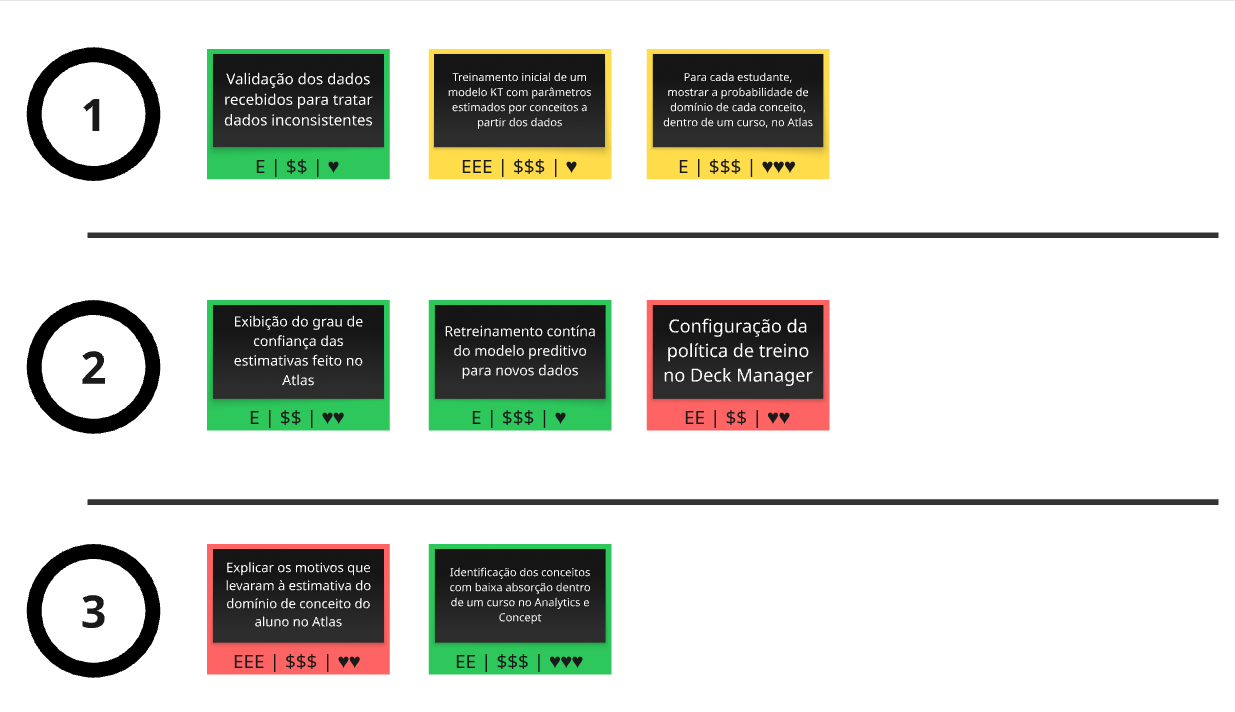
\includegraphics[width=\textwidth]{figuras/sequenciador1.png}
\legend{Fonte: Dos autores.}
\end{figure}

\begin{figure}[H]
\caption{Sequenciador do Cognita (ondas 4 a 6)}
\label{fig:ondas-mvp-2}
\centering
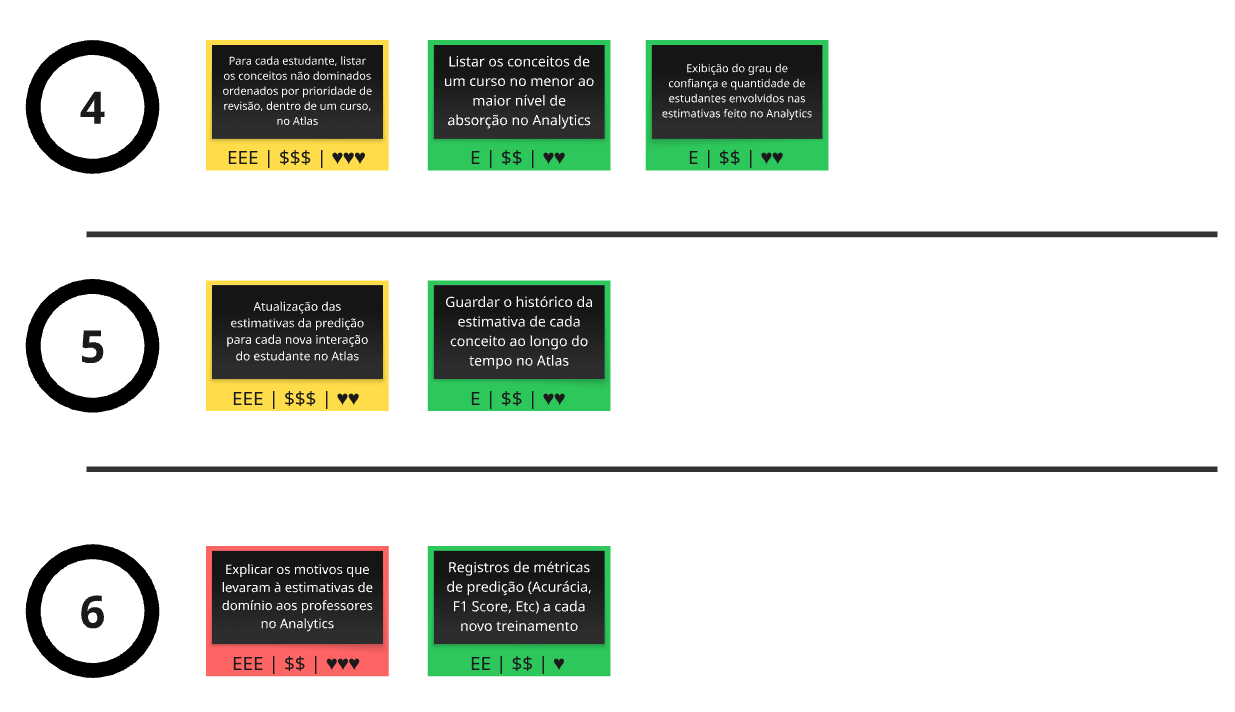
\includegraphics[width=\textwidth]{figuras/sequenciador2.png}
\legend{Fonte: Dos autores.}
\end{figure}

\begin{figure}[H]
\caption{Sequenciador do Cognita (ondas 7 a 10 e marcos do MVP e do incremento)}
\label{fig:ondas-mvp-3}
\centering
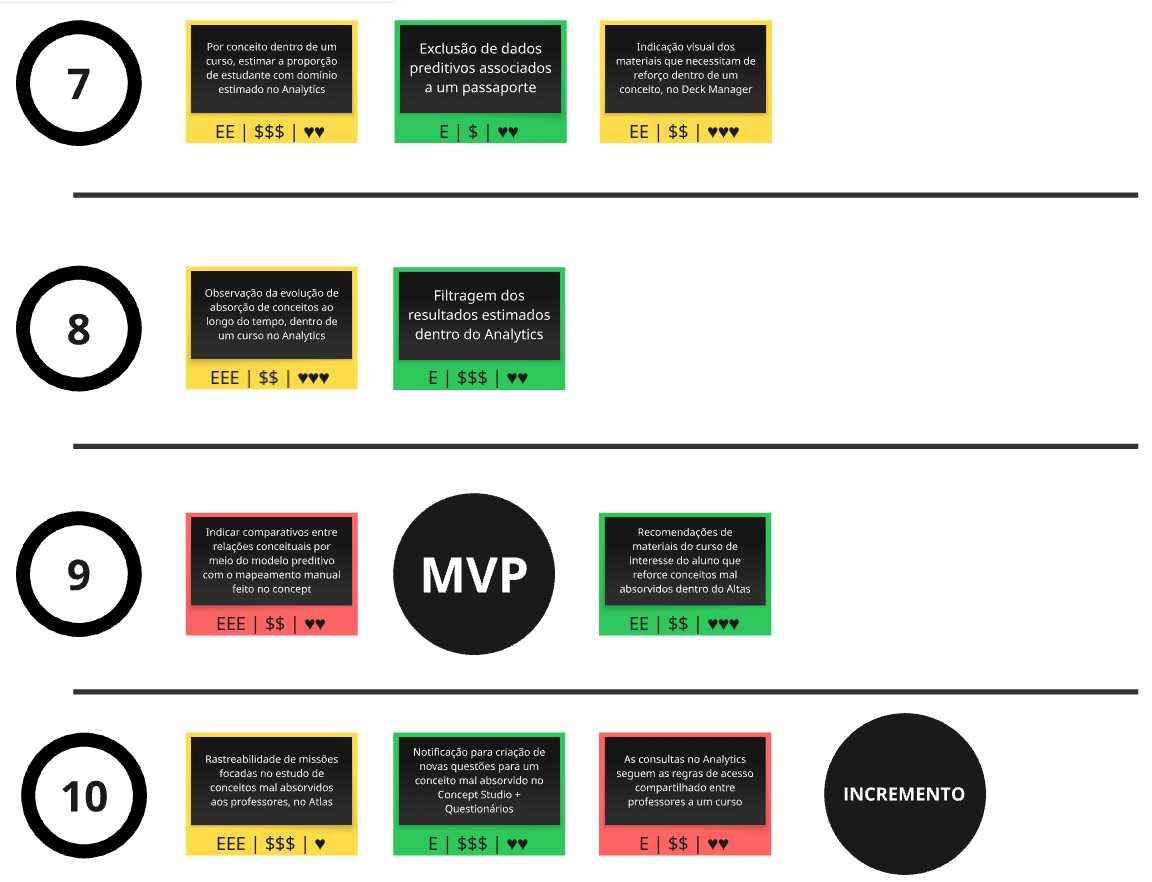
\includegraphics[width=0.9\textwidth]{figuras/sequenciador3.png}
\legend{Fonte: Dos autores.}
\end{figure}

A distribuição dos requisitos entre as ondas seguiu as seis regras do
sequenciador \cite{caroli_lean_2018}, apresentadas a seguir. Nelas, o
esforço, o valor agregado e a experiência do usuário de um requisito
correspondem à quantidade de símbolos \textit{E}, \$ e $\heartsuit$ de seu
cartão, de um a três.

\begin{enumerate}
    \item \textbf{Limite de requisitos:} uma onda pode conter, no máximo, três requisitos;
    \item \textbf{Limite de dificuldade:} uma onda não pode conter mais de um requisito de cor vermelha, isto é, de difícil aplicabilidade;
    \item \textbf{Equilíbrio de aplicabilidade:} uma onda com três requisitos não pode ser composta apenas por requisitos amarelos ou vermelhos, devendo conter ao menos um requisito verde;
    \item \textbf{Limite de esforço:} a soma do esforço dos requisitos de uma onda não pode ultrapassar cinco \textit{E};
    \item \textbf{Contribuição mínima de valor:} a soma do valor agregado dos requisitos de uma onda deve ser de, no mínimo, quatro \$, e a soma da contribuição para a experiência do usuário deve ser de, no mínimo, quatro $\heartsuit$, de modo que cada onda entregue valor de negócio e de UX relevantes;
    \item \textbf{Dependências:} se um requisito depende de outro, o requisito do qual ele depende deve estar em uma onda anterior.
\end{enumerate}

Para facilitar a leitura do sequenciador, a Tabela~\ref{tab:mvp-incrementos}
lista os requisitos de cada escopo, pelos seus códigos, com a onda em que
serão entregues.

{\small
\begin{longtable}{>{\raggedright\arraybackslash}p{1.6cm}>{\raggedright\arraybackslash}p{10.2cm}>{\centering\arraybackslash}p{1.6cm}}
\caption{Requisitos do MVP e do incremento do Cognita}
\label{tab:mvp-incrementos} \\
\hline
\textbf{Código} & \textbf{Requisito} & \textbf{Onda} \\
\hline
\endfirsthead
\caption[]{Requisitos do MVP e do incremento do Cognita (continuação)} \\
\hline
\textbf{Código} & \textbf{Requisito} & \textbf{Onda} \\
\hline
\endhead
\hline
\multicolumn{3}{r}{\textit{Continua na próxima página}} \\
\endfoot
\hline
\multicolumn{3}{l}{Fonte: Dos autores.} \\
\endlastfoot
\multicolumn{3}{l}{\textbf{MVP}} \\
\hline
RF01 & Treinamento inicial do modelo KT & 1 \\
\hline
RF03 & Validação dos dados recebidos & 1 \\
\hline
RF06 & Probabilidade de domínio por conceito & 1 \\
\hline
RF02 & Retreinamento contínuo do modelo & 2 \\
\hline
RF04 & Configuração da política de treino & 2 \\
\hline
RF16 & Grau de confiança das estimativas no Atlas & 2 \\
\hline
RF12 & Identificação de conceitos com baixa absorção & 3 \\
\hline
RF17 & Explicação da estimativa no Atlas & 3 \\
\hline
RF08 & Conceitos priorizados para revisão & 4 \\
\hline
RF13 & Listagem de conceitos por nível de absorção & 4 \\
\hline
RF18 & Confiança e amostra das estimativas no Analytics & 4 \\
\hline
RF07 & Atualização das estimativas por interação & 5 \\
\hline
RF09 & Histórico das estimativas por conceito & 5 \\
\hline
RF05 & Registro de métricas de predição & 6 \\
\hline
RF19 & Explicação da estimativa no Analytics & 6 \\
\hline
RF11 & Proporção de estudantes com domínio & 7 \\
\hline
RF20 & Indicação visual de materiais para reforço & 7 \\
\hline
RF24 & Exclusão de dados preditivos de um passaporte & 7 \\
\hline
RF10 & Evolução da absorção ao longo do tempo & 8 \\
\hline
RF15 & Filtragem dos resultados estimados & 8 \\
\hline
RF14 & Comparativo entre relações conceituais & 9 \\
\hline
\multicolumn{3}{l}{\textbf{Incremento}} \\
\hline
RF23 & Recomendação de materiais de reforço & 9 \\
\hline
RF21 & Notificação para criação de novas questões & 10 \\
\hline
RF22 & Rastreabilidade de missões de reforço & 10 \\
\hline
RF25 & Controle de acesso às consultas do Analytics & 10 \\
\hline
\end{longtable}
}

\section{Arquitetura}
\label{sec:arquitetura}

Esta seção documenta o estado atual da arquitetura do Ecossistema CEDIS e a
forma como o Cognita se integrará a ela. A caracterização dos produtos e da
arquitetura de dados foi apresentada na Seção~\ref{sec:dados-coletados}
e é aqui retomada sob a ótica de integração.

\subsection{Arquitetura Atual do Ecossistema}
\label{subsec:arquitetura-atual}

A Figura~\ref{fig:arquitetura-atual} representa o estado da arte do
ecossistema: os produtos e os serviços que o compõem, seus fluxos de dados
e os pontos em que o Cognita poderá obter informação.

% Futuramente: diagrama (ex.: C4 nível 1/2) com Navegador, Deck Manager, CEDIS Slides (slides-api),
% LA Ingest, Identity Suite (Learning Passport), Atlas / Concept Studio, Learning Analytics e cedis-core.
\begin{figure}[H]
\caption{Arquitetura atual do Ecossistema CEDIS}
\label{fig:arquitetura-atual}
\centering
\espacofigura[8cm]{Futuramente será inserido o diagrama da arquitetura atual do ecossistema}
\legend{Fonte: Dos autores.}
\end{figure}

\subsection{APIs do Ecossistema}
\label{subsec:apis-ecossistema}

A Tabela~\ref{tab:apis-ecossistema} lista as APIs e os serviços do
ecossistema relevantes para o Cognita, com a responsabilidade de cada um e
os dados que podem ser consumidos. A integração utiliza os protocolos de
autenticação e assinatura já adotados no ecossistema (OAuth2, OIDC e HMAC).

% Futuramente: APIs e serviços relevantes e seus endpoints/contratos.
\begin{table}[H]
\caption{APIs e serviços do ecossistema relevantes para o Cognita}
\label{tab:apis-ecossistema}
\centering
\begin{tabularx}{\textwidth}{>{\raggedright\arraybackslash}p{2.8cm}>{\raggedright\arraybackslash}X>{\raggedright\arraybackslash}X>{\raggedright\arraybackslash}p{2.4cm}}
\hline
\textbf{API / Serviço} & \textbf{Responsabilidade} & \textbf{Dados relevantes ao Cognita} & \textbf{Endpoints / contrato} \\
\hline
-- & -- & -- & -- \\
\hline
-- & -- & -- & -- \\
\hline
-- & -- & -- & -- \\
\hline
\end{tabularx}
\legend{Fonte: Elaborado pelos autores a partir do levantamento técnico apresentado na Seção~\ref{sec:dados-coletados}.}
\end{table}

\subsection{Arquitetura Proposta para o Cognita}
\label{subsec:arquitetura-proposta}

A Figura~\ref{fig:arquitetura-cognita} apresenta a integração proposta do
Cognita ao ecossistema: as fontes de dados consumidas, o \textit{pipeline}
de engenharia de atributos, o componente de estimativa de domínio e as
interfaces de entrega de \textit{feedback} a alunos e docentes.

% Futuramente: diagrama destacando o Cognita (ingestão, feature engineering,
% modelo de Knowledge Tracing, armazenamento do estado de domínio, API de consulta).
\begin{figure}[H]
\caption{Arquitetura proposta do Cognita integrada ao ecossistema}
\label{fig:arquitetura-cognita}
\centering
\espacofigura[8cm]{Futuramente será inserido o diagrama da arquitetura proposta do Cognita}
\legend{Fonte: Dos autores.}
\end{figure}


\section{Modelagem de Dados}
\label{sec:modelagem-dados}

Esta seção identifica os dados existentes no ecossistema que alimentarão o
Cognita e apresenta a modelagem das entidades e dos atributos envolvidos.

\subsection{Entidades e Atributos Utilizados}
\label{subsec:entidades-utilizadas}

A Tabela~\ref{tab:entidades-cognita} seleciona, dentre as entidades
descritas na Seção~\ref{subsec:modelo-dados}, aquelas que serão
consumidas pelo Cognita, indicando o componente de origem, os atributos
utilizados e a finalidade de cada uma.

% Futuramente: entidades e nomes reais dos campos de cada componente.
\begin{table}[H]
\caption{Entidades do ecossistema utilizadas como entrada do Cognita}
\label{tab:entidades-cognita}
\centering
\begin{tabularx}{\textwidth}{l>{\raggedright\arraybackslash}p{2.6cm}>{\raggedright\arraybackslash}X>{\raggedright\arraybackslash}X}
\hline
\textbf{Entidade} & \textbf{Origem} & \textbf{Atributos utilizados} & \textbf{Finalidade no Cognita} \\
\hline
-- & -- & -- & -- \\
\hline
-- & -- & -- & -- \\
\hline
-- & -- & -- & -- \\
\hline
\end{tabularx}
\legend{Fonte: Elaborado pelos autores a partir do levantamento técnico apresentado na Seção~\ref{sec:dados-coletados}.}
\end{table}


\section{Prototipação das Telas}
\label{sec:prototipacao}

A prototipação tem por objetivo validar, antes da implementação, os fluxos
de interação do aluno e do docente com o diagnóstico de domínio. A
Figura~\ref{fig:prototipo-telas} reúne os protótipos simples das telas do
Cognita, orientados aos requisitos funcionais da
Seção~\ref{subsec:requisitos-funcionais}.

% Futuramente: protótipos (telas do aluno e do docente), indicando os RF atendidos por cada tela.
\begin{figure}[H]
\caption{Protótipo das telas do Cognita}
\label{fig:prototipo-telas}
\centering
\espacofigura[10cm]{Futuramente serão inseridos os protótipos das telas}
\legend{Fonte: Dos autores.}
\end{figure}


\section{Cronograma de Desenvolvimento}
\label{sec:cronograma}

O desenvolvimento do Cognita será conduzido em onze \textit{sprints}. As
nove primeiras correspondem às ondas do MVP definidas no sequenciador da
\textit{Lean Inception} (Seção~\ref{subsec:mvp-incrementos}); os incrementos
não serão entregues no desenvolvimento. A décima \textit{sprint} é
reservada para testes e correções, e a última, para o congelamento de código
(\textit{code freeze}). A Tabela~\ref{tab:cronograma-ondas} associa cada
\textit{sprint} aos requisitos entregues, ao escopo da entrega e ao período
de execução.

{\small
\begin{longtable}{c>{\raggedright\arraybackslash}p{2.3cm}>{\raggedright\arraybackslash}p{6.3cm}cc}
\caption{Cronograma de desenvolvimento por \textit{sprints}}
\label{tab:cronograma-ondas} \\
\hline
\textbf{\textit{Sprint}} & \textbf{Requisitos (código)} & \textbf{Escopo da entrega} & \textbf{Início} & \textbf{Término} \\
\hline
\endfirsthead
\caption[]{Cronograma de desenvolvimento por \textit{sprints} (continuação)} \\
\hline
\textbf{\textit{Sprint}} & \textbf{Requisitos (código)} & \textbf{Escopo da entrega} & \textbf{Início} & \textbf{Término} \\
\hline
\endhead
\hline
\multicolumn{5}{r}{\textit{Continua na próxima página}} \\
\endfoot
\hline
\multicolumn{5}{l}{Fonte: Dos autores.} \\
\endlastfoot
1 & RF01, RF03, RF06 & Validação dos dados, treinamento inicial do modelo e probabilidade de domínio no Atlas. & 15/02/2027 & 25/02/2027 \\
\hline
2 & RF02, RF04, RF16 & Retreinamento e política de treino do modelo; confiança das estimativas no Atlas. & 26/02/2027 & 09/03/2027 \\
\hline
3 & RF12, RF17 & Explicação das estimativas no Atlas e identificação de conceitos com baixa absorção. & 10/03/2027 & 20/03/2027 \\
\hline
4 & RF08, RF13, RF18 & Conceitos a revisar no Atlas; ranking de absorção e confiança das estimativas no Analytics. & 22/03/2027 & 01/04/2027 \\
\hline
5 & RF07, RF09 & Atualização das estimativas por interação e histórico por conceito. & 02/04/2027 & 13/04/2027 \\
\hline
6 & RF05, RF19 & Métricas de predição por treinamento e explicação das estimativas no Analytics. & 14/04/2027 & 24/04/2027 \\
\hline
7 & RF11, RF20, RF24 & Proporção de estudantes com domínio, materiais para reforço e exclusão de dados do passaporte. & 26/04/2027 & 06/05/2027 \\
\hline
8 & RF10, RF15 & Evolução da absorção ao longo do tempo e filtros de resultados no Analytics. & 07/05/2027 & 18/05/2027 \\
\hline
9 & RF14 & Comparativo entre relações conceituais do modelo e do mapeamento manual, concluindo o MVP. & 19/05/2027 & 29/05/2027 \\
\hline
10 & -- & Reservada para testes e correções. & 31/05/2027 & 10/06/2027 \\
\hline
11 & -- & \textit{Code freeze}. & 11/06/2027 & 22/06/2027 \\
\hline
\end{longtable}
}
